\documentclass[twocolumn]{article}
%\documentclass[11pt]{article}
\usepackage[utf8]{inputenc}
\usepackage{enumerate}
\usepackage{amssymb}
\usepackage{amsfonts}
\usepackage{tikz}

%new command
\newcommand{\dkpoly}{$(d,k)$-polytope }

\begin{document}

%titre
\title{Idées de preuve que les (\textit{d},2)-polytopes sont Hirsch}
\author{Rado Rakotonarivo}
\maketitle

Dans le rapport précédent, les premières idées de preuves et une approche assez rudimentaire du problème ont été formulées. Ce rapport portera sur un bref rappel des résultats sur lesquels on va s'inspirer ainsi que sur l'établissement du contexte d'une manière plus concise, une reformulation plus claire du problème à résoudre: prouver Hirsch pour $k = 2$.

\section{Résultats antérieurs}
Del Pia et Michini trouvent dans \cite{del2016diameter} une borne supérieure pour le diamètre des $(d,k)$-polytopes pour $k\geq{2}$:

$$
	\delta\leq{\lfloor{(k-\frac{1}{2})}d\rfloor}
$$

Pour n'importe quelle valeur de $d$, il existe un $(d,2)$-polytope qui atteint cette borne.

Leur preuve s'appuie sur une méthode de récurrence sur la dimension en construisant un chemin reliant deux sommets $u$ et $v$ du \dkpoly sur son graphe. 

Soient donc $P$ un \dkpoly , $u$ et $v$ deux sommets de $P$. On note par $\delta(u,v)$ la distance au sens du graphe de $u$ et de $v$, et $\delta(P)$ le diamètre de $P$. Les sommets $u$ et $v$ sont choisis de telle manière qu'ils réalisent le diamètre, i.e. $\delta(P)\leq{\delta(u,v)}$.

Le principe est assez simple: ils proposent de trouver une face $F$ de $P$ réalisant un minimum suivant un hyperplan $c$ de l'espace ambiant. En posant $\gamma = \min\{cx:x \in P \}$, la face $F$ est définie comme suit $F = \{x \in P: cx = \gamma\}$. Par exemple, minimiser sur une dimension/direction revient à choisir $c=e^i$.

Pour borner $\delta(u,v)$, il suffit de borner la $\delta(u,F)$ et de la même manière borner $\delta(v,F)$. En utilisant la définition de $F$, on a:

\begin{equation}
	\delta(u,F)\leq{cu - \gamma}
\end{equation}

Comme $\delta(u,v)\leq{\delta(u,F) + \delta(v,F) + \delta(F)}$, on a:

\begin{equation}
	\delta(u,v)\leq{\delta(F) + cu + cv -2\gamma}
\end{equation}

La construction du chemin entre $u$ et $v$ consiste alors à construire récursivement un chemin partant respectivement de $u$ et de $v$ vers la face $F$. Et comme $F$ est une face de $P$, elle sera au plus de dimension $d-1$.

Il est explicité dans \cite{del2016diameter} que pour prouver leur résultat, il est suffit de prouver l'une de ces deux inégalités:

\begin{equation}
	\delta(u,v)\leq{\delta(d-1,k) + k -1}
\end{equation}
\begin{equation}	
	\delta(u,v)\leq{\delta(d-2,k) + 2k -1}
\end{equation}



\begin{center}
	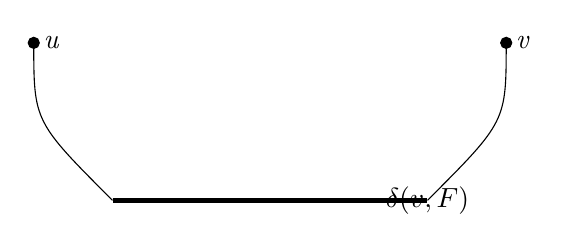
\begin{tikzpicture}
		\draw [ultra thick](-2,-2) -- (2,-2);
		\filldraw (-3,0) circle (2pt) node[anchor=west] {\textit{u}};
		\filldraw (3,0) circle (2pt) node[anchor=west] {\textit{v}};
		\draw (-3,0) .. controls (-3,-1) .. (-2,-2);
		\draw (3,0) .. controls (3,-1) .. (2,-2)node[anchor=center] {$\delta(v,F)$};
	\end{tikzpicture}
\end{center}






%Cette section va détailler les différentes étapes de la construction du chemin entre les sommets $u$ et $v$ pour finalement prouver le résultat.



\begin{enumerate}[i]
\item \textbf{Premier cas:}
$u+v=k^d$


\end{enumerate}

\begin{thebibliography}{9}
\bibitem{deza2016improved}
	Antoine Deza, Lionel Pournin.
	\emph{Improved bounds on the diameter of lattice polytopes}.
	arXiv preprint arXiv:1610.00341.
	2016.
\bibitem{naddef1989hirsch}
	Denis Naddef.
	\emph{The Hirsch conjecture is true for (0, 1)-polytopes}.
	Mathematical Programming, Springer.
	1989.
\bibitem{del2016diameter}
	Alberto Del Pia, Carla Michini.
	\emph{On the diameter of lattice polytopes}.
	Discrete \& Computational Geometry, Springer.
	2016.
\end{thebibliography}


\end{document}
